\documentclass[a4paper]{article}
\usepackage[margin=1in]{geometry}%设置边距,符合Word设定
\usepackage{amssymb,amsfonts,amsmath,amsthm}
\usepackage{ctex}
\usepackage{setspace}
\usepackage{lipsum}
\usepackage{graphicx}%插入图片
\graphicspath{{Figures/}}%文章所用图片在当前目录下的 Figures目录

\usepackage{hyperref} % 对目录生成链接,注:该宏包可能与其他宏包冲突,故放在所有引用的宏包之后
\hypersetup{colorlinks = true,  % 将链接文字带颜色
	bookmarksopen = true, % 展开书签
	bookmarksnumbered = true, % 书签带章节编号
	pdftitle = 第二章扩展作业(第二部分), % 标题
	pdfauthor = 刘正浩 2019270103005} % 作者

%\renewcommand{\contentsname}{\centerline{Contents}} %经过设置word格式后,将目录标题居中


\title{\heiti\zihao{2} 第二章扩展作业(第二部分)}
\author{\songti 刘正浩 2019270103005}
\date{2021.5.7}


\begin{document}
	\maketitle
	\thispagestyle{empty}

	%\begin{abstract}
	%	\lipsum[2]
	%\end{abstract}

	\tableofcontents

	\section{第一题}
		\begin{figure}[htbp]
			\centering
			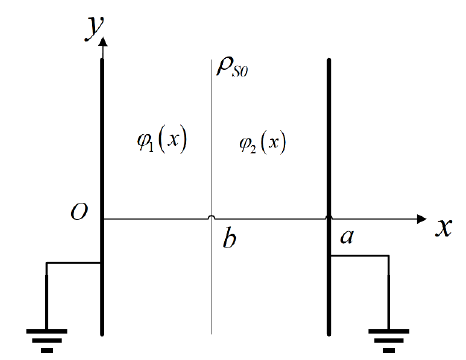
\includegraphics[scale=0.8]{1.png}
			\caption{平板与坐标系}
		\end{figure}
		在$x=b$两侧有电位函数:
		\begin{equation}
			\begin{split}
				\varphi_1 &= \varphi_1(x)\\
				\varphi_2 &= \varphi_2(x)
			\end{split}
		\end{equation}
		由于在分界面上没有自由电荷,所以泊松方程退化为拉普拉斯方程。
		\begin{equation}
			\begin{split}
				\nabla^2 \varphi_1(x) &= 0\\
				\nabla^2 \varphi_2(x) &= 0
			\end{split}
		\end{equation}
		方程的解为:
		\begin{equation}
			\begin{split}
				\varphi_1(x) &= C_1 x + D_1\\
				\varphi_2(x) &= C_2 x + D_2
			\end{split}
		\end{equation}
		利用边界条件,可知
		\begin{equation}
			\begin{split}
				x = 0处&,\varphi_1(0) = 0\\
				x = a处&,\varphi_2(a) = 0\\
				x = b处&,\varphi_1(b) = \varphi_2(b)\\
				\bigg[ \frac{\partial\varphi_2(x)}{\partial x} &- \frac{\partial\varphi_1(x)}{\partial x} \bigg]_{x=b} = -\frac{\rho_{S0}}{\epsilon_0}
			\end{split}
		\end{equation}
		由上面四个式子,将$\varphi_1(x)$与$\varphi_2(x)$带入解得
		\begin{equation}
			\begin{split}
				C_1 &= -\frac{\rho_{S0}(b-a)}{\epsilon_0 a}x\\
				C_2 &= -\frac{\rho_{S0}b}{\epsilon_0 a},\\
				D_1 &= 0\\
				D_2 &= \frac{\rho_{S0}b}{\epsilon_0}
			\end{split}
		\end{equation}
		最后得到
		\begin{equation}
			\begin{split}
				\varphi_1(x) &= \frac{\rho_{S0}(a-b)}{\epsilon_0 a}x\\
				\varphi_2(x) &= \frac{\rho_{S0}b}{\epsilon_0 a}(a-x)\\
				\vec{E}_1(x) &= -\nabla\varphi_1(x) = -\frac{\rho_{S0}(a-b)}{\epsilon_0 a} \cdot \vec{e}_x\\
				\vec{E}_2(x) &= -\nabla\varphi_2(x) = \frac{\rho_{S0}b}{\epsilon_0 a} \cdot \vec{e}_x
			\end{split}
		\end{equation}

\end{document}